\section{Theorie}
\label{sec:Theorie}

Da \textit{RC-Kreise} immer eine gewisse Zeit brauchen um sich aufzuladen, beziehungsweise zu entladen,
müssen diese Prozesse natürlich auch mathematisch beschrieben werden.
Im folgenden sind die wichtigsten Formeln zusammengefasst \cite[1-5]{v353}.

\subsection{Allgemeine Relaxionsgleichung}
Es wird davon ausgegangen dass es eine Größe $A$ gibt, die ein Supremum bei der Auf/- und Entladung besitzt.
Das bedeutet, es gibt eine Änderungsgeschwindigkeit, die sich für große t gegen null bewegen muss, da
$A(t)$ immer weiter gegen $\text{sup}(A(t))$ strebt.
Es zeichnet sich also ein asymptotisches Verhalten ab.
Die allgemeine Änderungsgeschwindigkeit wird durch
\begin{equation}
    \frac {dA}{dt} = c \left[ A(t) - A(\infty) \right]
\end{equation}
beschrieben, wobei $c$ eine Konstante ist.
Außerdem gilt
\begin{equation}
A(t) = A(\infty) + \left[ A(0) - A(\infty) \right] e^{ct} \, .
\end{equation}
Dabei ist jedoch zu beachten, dass für den beschränkten Fall, der ja hier interessant ist,
$c < 0$ sein muss, da sonst kein Supremum von $A$ vorliegt.


\subsection{Entladevorgang}
\begin{figure}
    \centering
    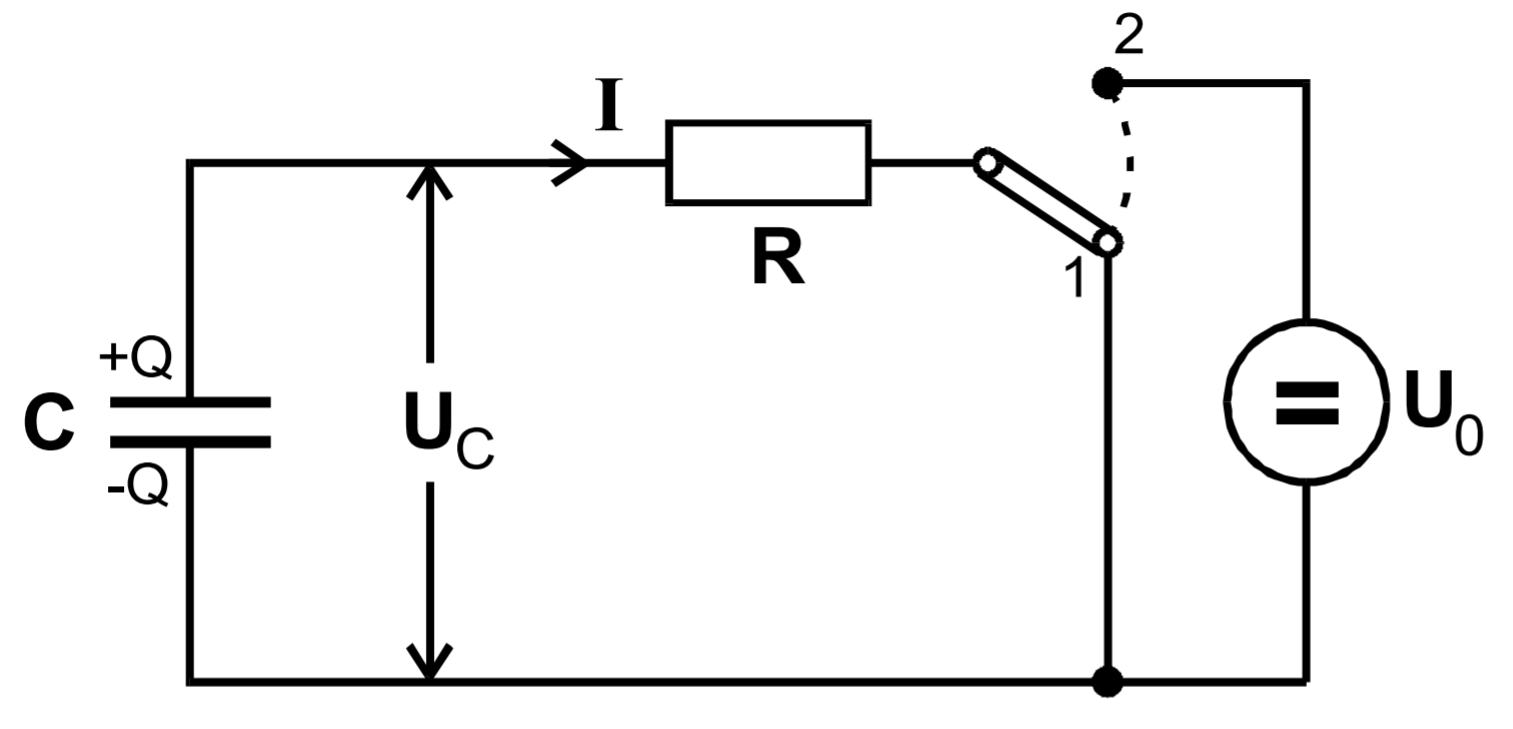
\includegraphics[width=0.5\textwidth]{pictures/Schaltung1.png}
    \caption{Schaltung mit Entladung in Pos. 1 und Aufladung in Pos. 2 \cite[1]{v353}.}
    \label{fig:Schaltung1}
\end{figure}

Eine beispielhafte Schaltung mit Auf/- und Entladevorgängen ist in Abbildung \ref{fig:Schaltung1} dargestellt.
Für die Entladung wird davon ausgegangen, dass er Schalter lange genug in Position 1, also dem Aufladevorgang war,
dass sich die Ladung $Q$ dort deponiert hat.
Dann gilt für die Kondensatorspannung
\begin{equation}
    U_\text{C} = \frac{Q}{C} \, ,
\end{equation}
wobei $C$ die kapazität des Kondensators beschreibt.
Nun wird durch das ohmsche Gesetz ein Strom angelegt. Es gilt
\begin{equation}
    I = \frac{U_\text{C}}{R} \, .
\end{equation}
Dabei ist $R$ ein ohmscher Widerstand.
Da nach Umlegung des Schalters Ladung abfließt, gilt
\begin{equation*}
    dQ = -I dt \, ,
\end{equation*}
woraus sich 
\begin{equation*}
    \frac{dQ}{dt} = -\frac{1}{R C} \cdot Q(t)
\end{equation*}
ergibt. Da sich ein Grenzwert $Q(\infty) = 0$ einstellen wird, gilt
\begin{equation}
    Q(t) = Q(0) \cdot e^{- \frac{t}{R C}} \, .
\end{equation}

\subsection{Aufladevorgang}

Analog lässt sich auch die Aufladung beschreiben.
Es wird also davon ausgegangen, dass der Schalter in Abbildung \ref{fig:Schaltung1} eine große Zeit $t$ in
Position 2 war.
Nun gelten die Anfangsbedingungen
\begin{align*}
    Q(0) &= 0 & \text{und} & & Q(\infty) &= C U_0 \, .
\end{align*}
Der Aufladevorgang wird also durch die Gleichung 
\begin{equation}
    Q(t) = C U_0 (1 - e^{- \frac{t}{R C}})
\end{equation}
beschrieben.

\subsection{Relaxionsphänomene bei Wechselspannungen}
\begin{figure}
    \centering
    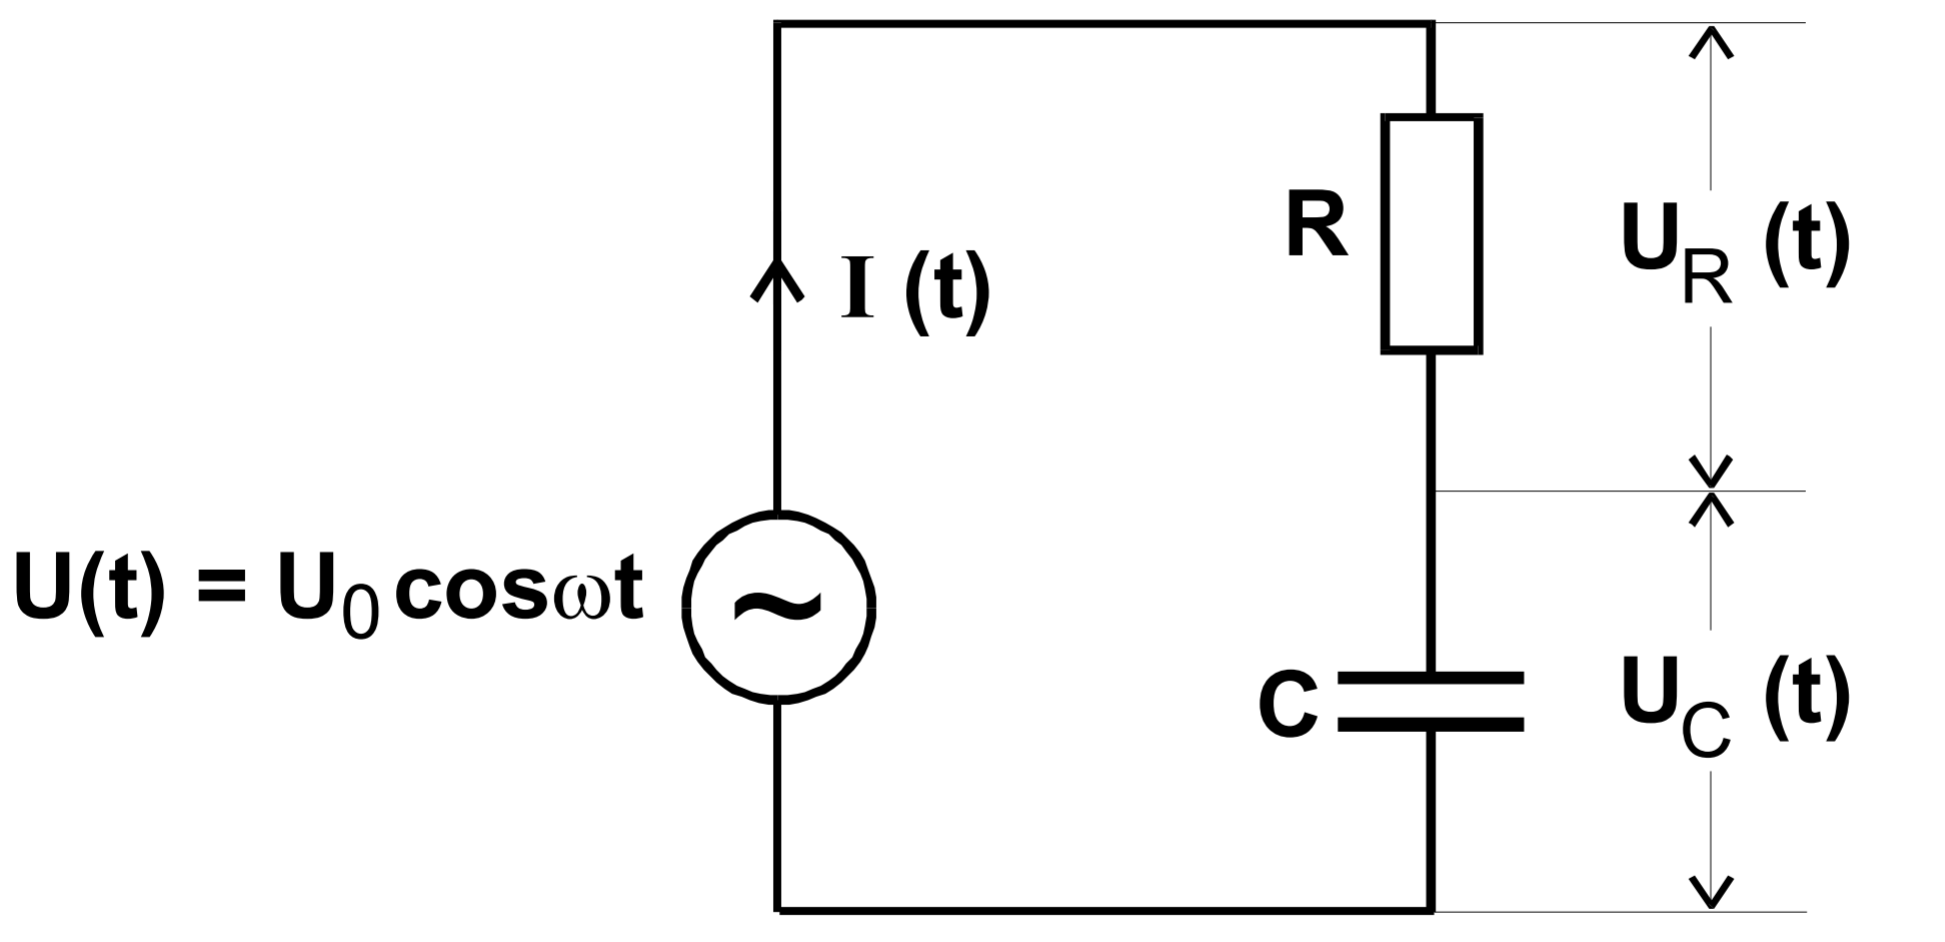
\includegraphics[width=0.5\textwidth]{pictures/Schaltung2.png}
    \caption{Beispielschaltung für Relaxionsphänomene bei einer Wechselspannung \cite[3]{v353}.}
    \label{fig:Schaltung2}
\end{figure}

Legt man eine Wechselspannung an, wie beispielsweise in Abbildung \ref{fig:Schaltung2}, dann kommt es zu
Relaxionsphänomenen.
Dabei wird durch die äußere Wechselspannung
\begin{equation}
    U(t) = U_0 \cdot cos(\omega t)
\end{equation}
der RC-Kreis weiter angeregt.
Dadurch wird sich eine Phasenverschiebung zwischen Generatorspannung und Kondensatorspannung ergeben.
Dieses problem versucht man dann durch den Ansatz
\begin{equation*}
    U_\text{C} = A(\omega) \cdot cos(\omega t + \phi(\omega))
\end{equation*}
zu lösen.
Nach etwaigen Umformungen und weiteren Annahmen gelangt man zu der Gleichung
\begin{equation}
    A(\omega) = \frac {U_0}{\sqrt{1 + \omega^2 R^2 C^2}} \, .
\end{equation}

\subsection{Integrationsverhalten eines RC-Kreises}
Unter bestimmten Bedingungen, kann ein RC-Kreis als Integrator dienen.
Dafür muss zunächst
\begin{equation*}
    \omega >> \frac {1}{R C}
\end{equation*}
erfüllt sein. Dann gilt
\begin{equation}
    U_\text{C} (t) = \frac{1}{R C} \int_0^t U(t')dt' \, .
\end{equation}